\section{Lineage Tracing}
\label{sec:lic}

As a foundation of lineage-based reuse, we first describe efficient means to lineage tracing and key operations. Lineage graphs may get very large though, especially for mini-batch training. For this reason, we introduce the idea of lineage deduplication for loops and functions. Finally, we discuss design decisions and limitations.

\subsection{Basic Lineage Tracing}
\label{sec:tracing}

During runtime of a linear algebra program, LIMA maintains---in a thread- and function-local manner---lineage DAGs for all live variables of this execution context. Figure~\ref{fig:lineage} shows the lifecycle of such lineage information and key operations.

\begin{definition2}[Lineage DAGs] A lineage DAG $\mathcal{L}$ is a directed, acyclic graph, whose nodes (or lineage items) represent operations and their outputs, and whose edges represent data dependencies. Lineage items consist of an ID, an opcode, an ordered list of input lineage items, an optional data string and hash, and a visited flag for memoization of processed sub graphs. Leaf nodes are literals or matrix creation operations (e.g., \texttt{read} or \texttt{rand}), and multiple inner nodes might refer to the same inputs. Thus, the lineage DAG is a data flow graph, that encodes the exact creation process of intermediate results, without the computation that determined the control flow path.
\end{definition2}

\textbf{Lineage Tracing:} The immutable lineage DAG for live variables is then incrementally built by lineage tracing as we execute runtime instructions (Figure~\ref{fig:lineage}, \emph{trace}). Every execution context maintains a \texttt{LineageMap} that maps live variable names to lineage items (Figure~\ref{fig:lineage}, red root nodes), and caches literal lineage items. As a lean runtime integration, individual instructions---in a class hierarchy of instructions for local and distributed operations---implement a dedicated interface \texttt{LineageTraceable} for obtaining lineage items. Before\footnote{Lineage tracing \emph{before} instruction execution facilities reuse as described in Section~\ref{sec:reuse}.} executing an instruction (integrated in \texttt{preprocessInstruction}), we obtain the lineage items for the instruction output(s) and update the lineage map. Special instructions like \texttt{mvvar} and \texttt{rmvar}---for renaming and removing variables---only modify the mapping of live variables to lineage items. For capturing non-determinism, we also modified selected runtime instructions, like \texttt{rand} or \texttt{sample}, to create system-generated seeds on \texttt{preprocessInstruction} for inclusion in the lineage items.

\textbf{Comparisons:} When working with multiple, potentially overlapping lineage DAGs, a key operation is the comparison of two lineage DAGs for equivalence or containment (Figure~\ref{fig:lineage}, \emph{compare}). For this purpose, lineage items implement \texttt{hashCode()} and \texttt{equals()}, whose semantics are recursively defined. First, the hash code of a lineage item is computed as a hash over the hashes of the opcode, data item, and all inputs. As lineage DAGs are immutable, we cache the computed hash for every lineage item. Second, the equals check returns true if the opcode, data item, and all inputs are equivalent. In order to handle large DAGs, we use memoization to avoid redundant processing of sub-DAGs reachable over multiple paths, and non-recursive, queue-based function implementations.  

\textbf{Serialization and Deserialization:} Users may obtain the lineage in two forms. First, a new \texttt{lineage(X)} built-in function returns the lineage DAG of variable $\mat{X}$ as a string. Second, for every write to a file \texttt{write(X,'f.bin')}, we also write the lineage DAG to a text file \texttt{'f.bin.lineage'}. Both cases require the serialization of the lineage DAGs (Figure~\ref{fig:lineage}, \emph{serialize}). This serialization unrolls the lineage DAG in a depth-first manner, creating a text line per lineage item. Inputs are represented via IDs and memoization ensures that every item is serialized once in the lineage log. To handle large DAGs, we again use a non-recursive implementation with stack-based data structures. The lineage log can be deserialized back into a lineage DAG (Figure~\ref{fig:lineage}, \emph{deserialize}) by processing the lineage log line-by-line. For every line, we obtain input items from a lookup table, create the lineage item, and store it in the lookup table.

\textbf{Re-computation from Lineage:} Additionally, we provide a utility for generating a runtime program from a lineage DAG (Figure~\ref{fig:lineage}, \emph{reconstruct}) that computes---given the same input---exactly the same intermediate. In contrast to the original program, the reconstructed program does not contain control flow but only the operations for computing the output. The entire lifecycle from tracing, over serialization and deserialization, to the re-computation by lineage is very valuable as it simplifies testing, debugging, and reproducibility as illustrated by the following example.

\begin{example}[Debugging with Lineage] Let us share a debugging story from practice, which motivated the lineage support in SystemDS. Users deployed a sentence classification pipeline in production, noticed differences in results compared to the development setup, and reported this as a blocking issue. We reproduced the setup, spent nights debugging it up to round-off errors of different degrees of parallelism, and yet, still could not reproduce it. Finally, we found that the modified deployment infrastructure passed arguments incorrectly, making the pipeline use default parameters. With lineage support, such multi-person debugging efforts become much simpler: lineage logs can be exchanged, compared, and used to reproduce results.
\end{example}

\begin{figure}[!t]
	\centering
	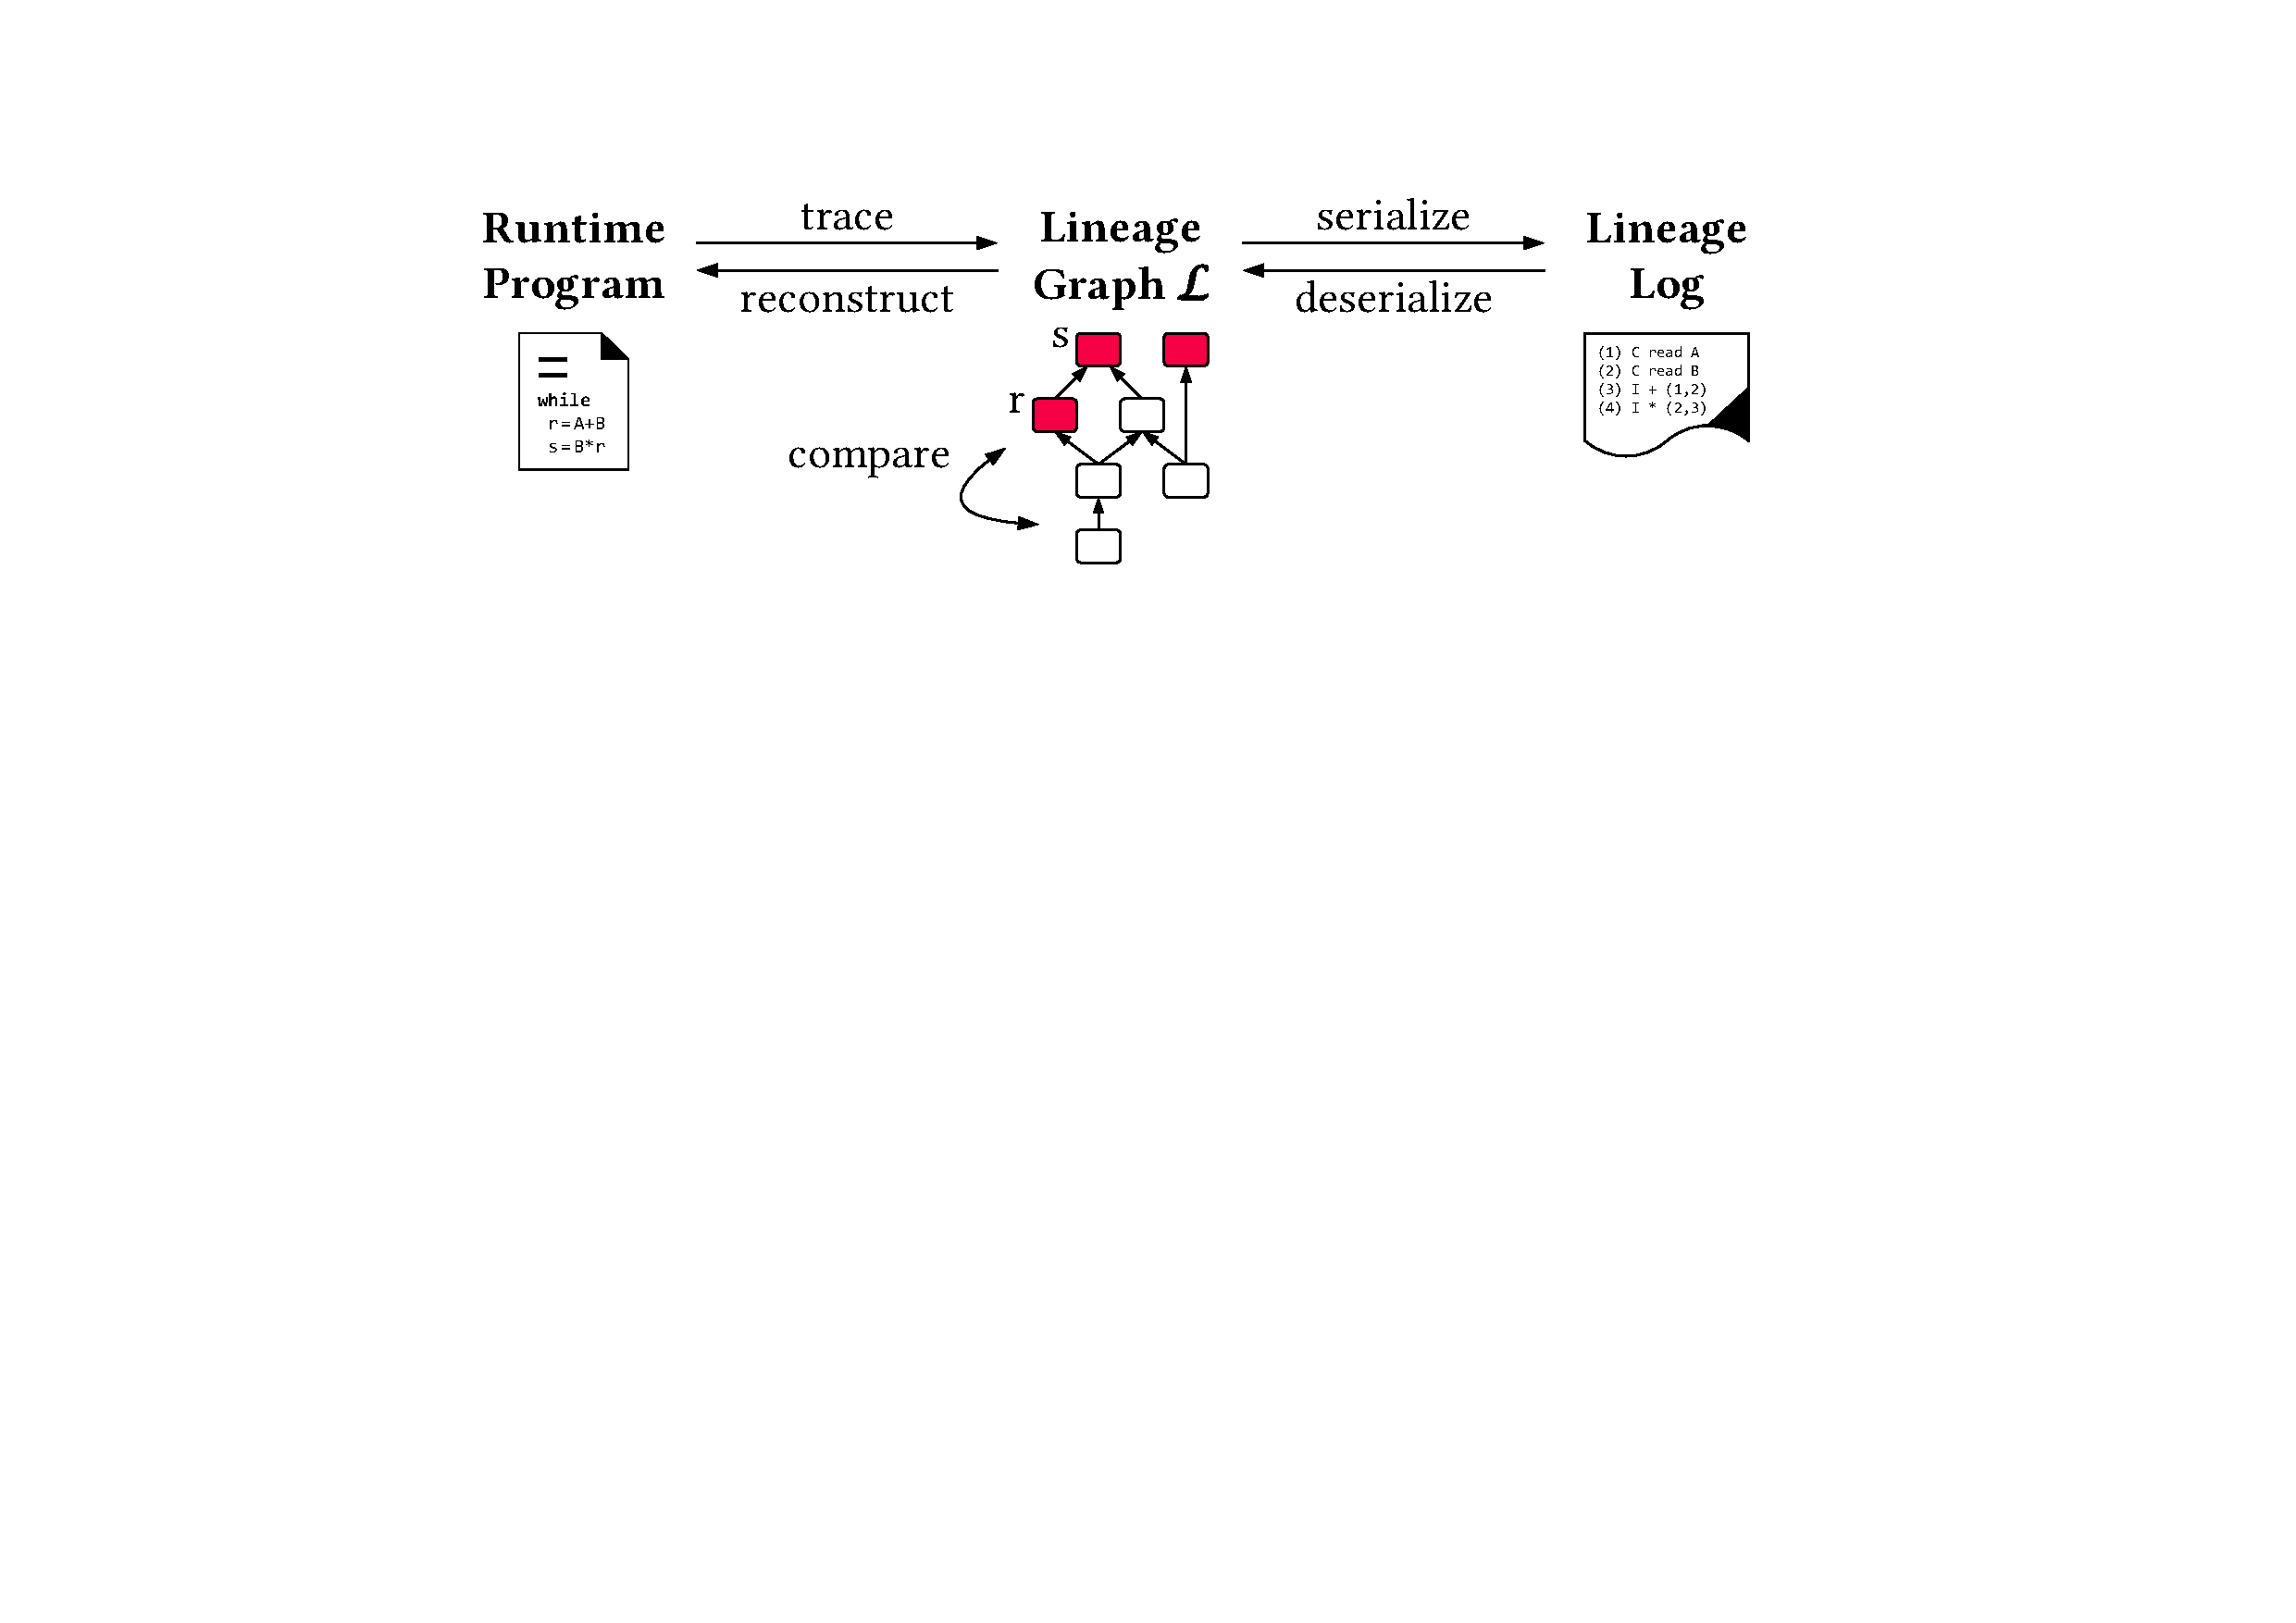
\includegraphics[scale=0.32]{figures/lineage}
	\vspace{-0.25cm}
	\caption{\label{fig:lineage}Lineage Tracing Lifecycle and Operations.}
\end{figure}

\subsection{Lineage Deduplication}
\label{sec:deduplication}

A new challenge of fine-grained lineage tracing are potentially very large lineage DAGs in use cases like mini-batch training. Consider an average lineage item size of $64\bb$, and training 200 epochs on a dataset of $10\text{M}$ rows, batch-size 32, and $\num{1000}$ instructions per iteration. The resulting lineage DAG would grow to $4\tb$. We address this issue inside ML systems with a new concept of \emph{lineage deduplication}, reducing the size to $4\gb$ in this example. Additionally, deduplication can remove the overhead of repetitive tracing.

\textbf{Basic Idea:} Large lineage DAGs originate from the repeated execution of code paths in loops and functions, which create repeated patterns in the lineage graph. The basic idea of lineage deduplication is to eliminate these repeated patterns in the lineage DAG as a form of compression. Conceptually, we extract lineage sub-DAGs called patches, store them once, and refer to these patches via a single lineage item. Since reactive deduplication (after lineage tracing)---similar to function outlining---is a hard problem and brittle, we perform proactive deduplication on entering last-level loops and functions. However, as the number of lineage patches is exponential in the number of branches, we use a \emph{hybrid} design with proactive setup, and minimal runtime tracing.

\textbf{Loop Deduplication Setup:} On entering a last-level \texttt{for}, \texttt{parfor}, or \texttt{while} loop, we analyze the distinct control paths to aid deduplication. The distinct control paths are all possible execution paths (e.g., $2^3$ paths for a sequence of three \texttt{if-else}-blocks), each with its own lineage patch. During setup, we count these paths in a single pass through the program, replicating the current set of traced paths at every branch. In this process, we also assign branch positions (IDs) and materialize these IDs in the \texttt{if-else} program blocks. For nested branches, the IDs are assigned in a depth-first order of the entire subprogram. Additionally, we obtain the inputs and outputs of the loop body from live variable analysis, and prepare an empty map of lineage patches but do not materialize these patches to avoid unnecessary setup for paths that are never taken.

\textbf{Loop Deduplication Tracing:} During iteration runtime, we trace temporary lineage DAGs. We first construct ordered placeholder items for the loop inputs and indexes. Additionally, we initialize a bitvector \mat{b} for tracing the taken path, where bit $\mat{b}_i$ is set to the evaluated condition of branch $i$. We then execute the loop body, while performing basic lineage tracing and updating \mat{b}. At the end of an iteration, we maintain the map of lineage patches and the global lineage DAG. The bitvector \mat{b} represents the key of the lineage patch, and we keep the collected lineage DAG as a new patch if it does not yet exist. Finally, a single dedup lineage item---pointing to the lineage patch---is added onto the global lineage DAG. Once lineage patches are created for all distinct paths, we stop this on-demand lineage tracing, and only trace the taken control paths.

\begin{figure}[!t]
	\centering
	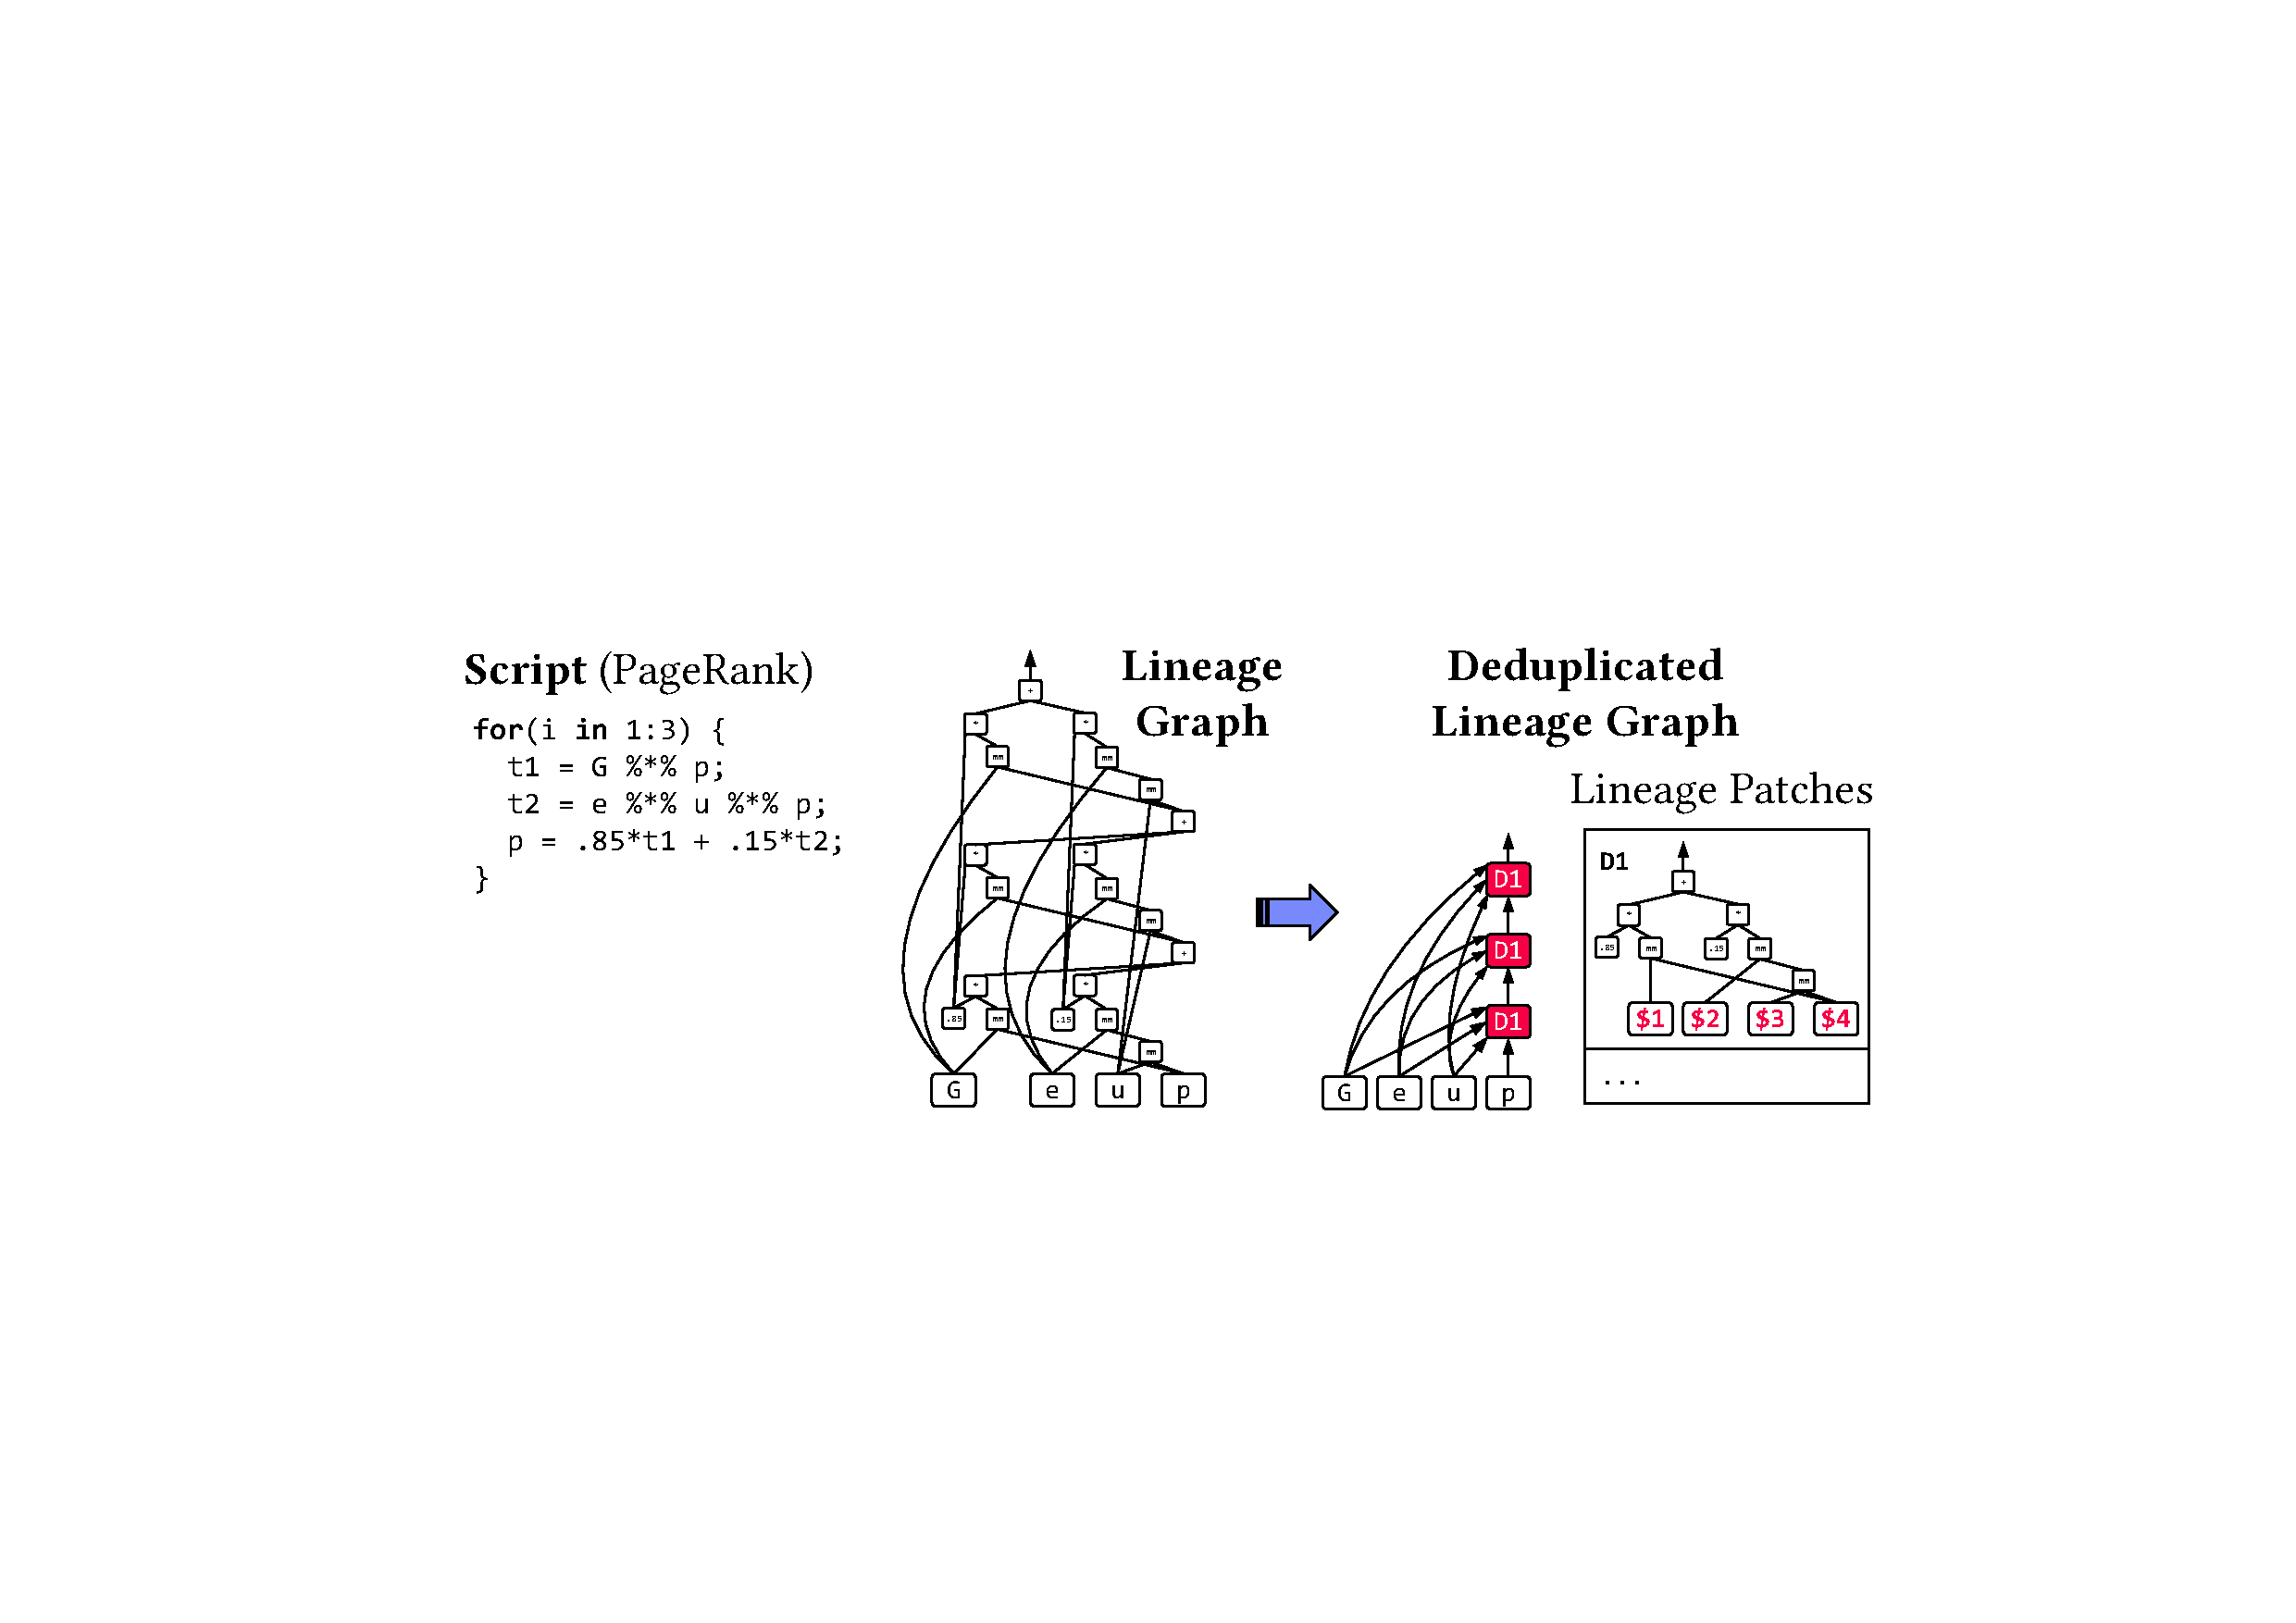
\includegraphics[scale=0.32]{figures/dedup}
	\vspace{-0.25cm}
	\caption{\label{fig:dedup}Example Lineage Deduplication for PageRank.}
\end{figure}

\begin{example}[PageRank Loop Deduplication] Figure~\ref{fig:dedup} illustrates this concept of loop deduplication for a classical PageRank graph algorithm. On the left, we see the original script, where $\mat{G}$ is a sparse graph representing the linked websites, and $\mat{p}$ is the iteratively updated page rank of individual sites. When executing three iterations without deduplication, we get the lineage graph in the center with repeated substructures. In contrast, with loop deduplication, we have extracted one lineage patch with four inputs and one output, and add a single lineage item per iteration to the lineage graph.
\end{example}

\textbf{Function Deduplication:} Similar to loop deduplication, we apply the same concept for functions that do not contain loops or other function calls. We again count the distinct control paths upfront, use the bitvector approach to trace the taken path, and add a single lineage item per function call to the lineage graph. Additional support for nested loops and function calls is interesting future work. We focused on last-level loops and functions, which offers a good tradeoff between simplicity and benefit of deduplication.

\textbf{Handling of Non-Determinism:} Coming back to our example of mini-batch training. Many DNN architectures contain \texttt{dropout} layers for regularization, which is a non-deterministic operation that generates new dropout masks in every iteration. Our approach to handling such non-determinism in the context of deduplication is to model the seeds as input placeholders of the lineage patch, trace these seeds like the control path bitvector, and add them as literal inputs to the single dedup item. Similarly, all functions are tagged as deterministic or non-deterministic during compilation.

\textbf{Operations on Deduplicated Graphs:} All basic lineage operations apply to deduplicated lineage graphs too. However, na\"ively decompressing the lineage graph---by lookup of lineage patches and expansion---would defeat the purpose of deduplication. We alleviate this problem by two extensions. First, we \emph{serialize} and \emph{deserialize} the dictionary of lineage patches to preserve the deduplication for storage and transfer. We further extended the \emph{compare} functionality to match normal and deduplicated sub-DAGs, by enforcing equal hashes for regular and dedup items, and resolving dedup items if needed. Second, program reconstruction would also cause expansion. Hence, on \emph{reconstruct}, we compile the lineage patches into functions, and sequences of equivalent dedup items into loops.

\subsection{Lineage Tracing for Advanced Features}
\label{sec:advanced}

Modern ML systems further provide advanced features such as (1) operator fusion, and (2) task-parallel for loops, which are both widely used and thus, important to integrate with lineage tracing.

\textbf{Operator Fusion:} Operator fusion via code generation is crucial for performance because it can avoid materialized intermediates \cite{CrottyGDKBCZ15,BoehmRHSEP18,PalkarTNTPNSSPA18}, allow scan sharing and sparsity exploitation \cite{BoehmRHSEP18,HuangB013}, and kernel specialization for accelerators \cite{ChenMJZYSCWHCGK18,XLA,AshariTBRCKS15}. However, fusion loses the operator semantics and thus, does not allow lineage tracing. This limitation is problematic because it cuts the lineage trace into unusable pieces. Our approach is simple, yet effective. We construct the lineage patches of fused operators (with ordered placeholders) during compilation, and store them in a dictionary. During runtime, we expand the lineage graph by these lineage patches. Lineage now also enables new techniques such as de-optimizing fused operators and reuse-aware fusion.
  
\textbf{Task-parallel Loops:} Numerical computing frameworks like MATLAB~\cite{SharmaM09}, R~\cite{Rdopar}, or Julia~\cite{BezansonEKS17}, and ML systems like TensorFlow~\cite{AbadiBCCDDDGIIK16} or SystemML~\cite{BoehmDEEMPRRSST16,BoehmTRSTBV14} provide means of task-parallel loops (e.g., for hyper-parameter tuning). Implementation details vary, but often multi-threaded and/or distributed workers are used. For ensuring isolation, we trace lineage in a worker-local manner, but individual lineage graphs share their common input lineage. Distributed operations leverage the \emph{serialize} and \emph{deserialize} operations to transfer lineage. The worker results are merged by taking their lineage roots and constructing a linearized lineage graph.

\subsection{Limitations}
\label{sec:limits1}

The LIMA lineage tracing makes several tradeoffs. In the following, we discuss these design decisions and related limitations.
\begin{itemize}
\item \emph{Immutable Files/RDDs:} We assume input files and RDDs are read-only (i.e., deterministic reads), which is a reasonable assumption and eliminates the need for data summarization. 
\item \emph{No Capturing of Control Flow:} The lineage DAG represents the computation of an intermediate without the control path decisions. We made this choice because the original script is a more concise representation of the actual program.
\item \emph{Result Differences:} Despite handling non-determinism, reconstructed programs might produce slightly different results. Reasons include multi-threaded or distributed operations (aggregation orders), different environments (memory budgets, cluster size), and different artifacts (SW versions).
\end{itemize}
Our design focuses primarily on simplicity, efficiency, and robustness, which are key for leveraging lineage in many use cases like versioning, debugging, auto differentiation, and lineage-based reuse. 

%TODO deduplication with non-determinism (seed placeholders) 
%TODO deduplication for functions
